\section{ХОД РАБОТЫ}

\subsection{Постановка задачи}

Написать оконное приложение, иллюстрирующее работу со списками.
Из списка выбирается название книги. Для выбранной книги из
файла считывается информация по ней и отображается в текстовом поле.

\subsection{Особенности рахработанного приложения}

В GTK для описания графического интерфейса могут использововаться xml-файлы.
Преимущество такого подхода заключается в том, что графический интерфейс,
описанный в xml-файле, не зависит от языка, на котором будут реализовываться
обработчики событий.

На рисунке~\ref{lst:xml_interface} представлен фрагмент описания графического 
интерфейса, сгенерированный приложением Glade.

\begin{lstlisting}[caption=Фрагмент описания графического интерфейса приложения,
label=lst:xml_interface,language={xml},basicstyle=\scriptsize\ttfamily]
<?xml version="1.0" encoding="UTF-8"?>
<glade-interface>
  <!-- interface-requires gtk+ 2.24 -->
  <!-- interface-naming-policy project-wide -->
  <widget class="GtkWindow" id="mainWindow">
    <property name="visible">True</property>
    ...
    <child>
      <widget class="GtkVBox" id="vbox1">
        <child>
          <widget class="GtkHButtonBox" id="hbuttonbox1">
            <child>
              <widget class="GtkButton" id="button1">
                <property name="label">gtk-open</property>
                <property name="visible">True</property>
                <property name="can_focus">True</property>
                <property name="receives_default">True</property>
                <property name="use_stock">True</property>
                <signal name="clicked" handler="onChooseBookDir" swapped="no"/>
              </widget>
              ...
\end{lstlisting}

Как видно, для представления элементов интерфейса используются XML-теги,
а для задания опций и сигналов --- атрибуты.

Для организации работы со списками в GTK используется виджет TreeView,
который в зависимости от типа используемого хранилища (storage) может
отображать информацию в виде списков или деревьев.

Программный код приложения состоит из двух классов: \texttt{BookShelfApp} и
\texttt{BookShelfModel}.

Класс \texttt{BookShelfApp} предоставляет реализации сигналов, 
заданных в xml-файле. Связывание сигналов с реализациями производится 
за счет вызова библиотечного метода \texttt{Autoconnect()}.

Вспомогателный класс \texttt{BookShelfApp} выполняет операции по наполнению
списка книг и получению содержания требуемой книги.

Интерфейс разработанного приложения представлен на рисунке~\ref{pic:interface}.

\begin{figure}[h!]
  \centering
  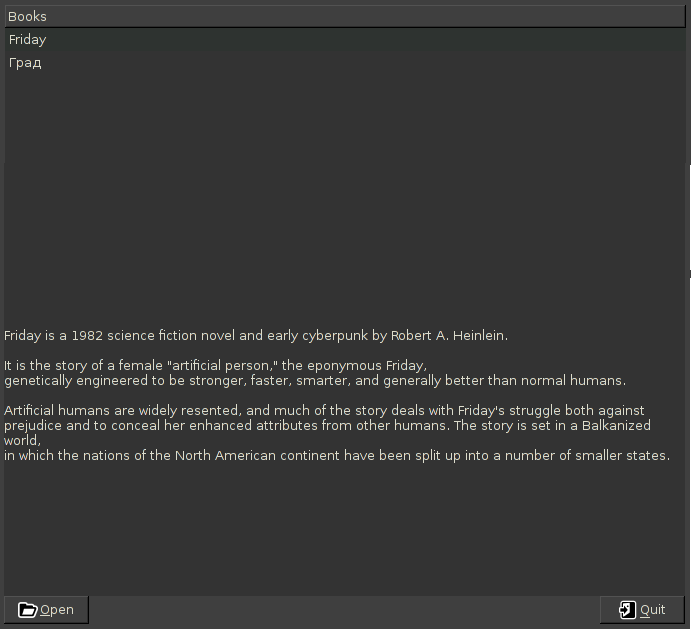
\includegraphics[width=150mm]{pic/interface}
  \caption{Интерфейс разработанного приложения}
  \label{pic:interface}
\end{figure}

Исходный текст разработанного приложения находится в приложении~А.